% NTCIR-19 CAMEO — team retrank — 6-minute talk (+2 min Q&A)
% Every number and claim here is taken from the submitted paper
% (docs/paper/ntcir19_cameo_retrank.tex); do not add results that are not in it.
\documentclass[aspectratio=169,10pt]{beamer}
\usetheme{default}
\usecolortheme{whale}
\useinnertheme{circles}
\setbeamertemplate{navigation symbols}{}
\setbeamertemplate{footline}[frame number]
\setbeamertemplate{itemize items}[circle]
\usepackage{booktabs}
\usepackage{xcolor}
\usepackage{tikz}
\usetikzlibrary{arrows.meta,positioning,calc}
\definecolor{accent}{RGB}{0,96,160}
\setbeamercolor{frametitle}{bg=accent,fg=white}
\setbeamercolor{title}{fg=white,bg=accent}
\setbeamercolor{subtitle}{fg=white}
\setbeamercolor{structure}{fg=accent}

\title[retrank @ CAMEO]{Metadata-Grounded Composed Image Retrieval\\for Vietnamese E-commerce}
\subtitle{Team \textbf{retrank} --- NTCIR-19 CAMEO CIR Subtask}
\author{Alessandro Magnani}
\institute{Independent}
\date{NTCIR-19, Tokyo, December 2026}

\begin{document}

{\setbeamertemplate{footline}{}
\begin{frame}[plain]
  \titlepage
  \begin{center}\small
  Two-stage pipeline \;$\cdot$\; \textbf{recall is the ceiling} \;$\cdot$\;
  metadata (esp.\ price) is a first-class signal \;$\cdot$\; competitive local VLM rerankers
  \end{center}
\end{frame}}

% ------------------------------------------------------------------
\begin{frame}{The task: Composed Image Retrieval for e-commerce}
\begin{columns}[T]
\begin{column}{0.56\textwidth}
Given a \textbf{reference product image} + a \textbf{natural-language
modification}, rank a fixed catalogue.
\medskip

\emph{``the same product but cheaper''} \\
\emph{``a gel cleanser from brand X''}
\medskip

\begin{itemize}
  \item Corpus: \textbf{4{,}086} Vietnamese skincare products
        (cleansers, toners, sunscreens, \dots), each with image, brand,
        price (VND), name/description
  \item \textbf{20} official CIR topics (Vietnamese shopper requests)
  \item Pooled 3-point human judgments; \textbf{nDCG@5 / nDCG@10}
\end{itemize}
\end{column}
\begin{column}{0.44\textwidth}
\footnotesize
\begin{block}{Why it's hard here}
Many requests are about \textbf{price, brand, format} --- attributes in the
product's text metadata, invisible to a purely visual encoder.
\end{block}
\begin{block}{How we measured (not comparable)}
\textbf{Dev-429}: our synthetic set, one exact answer per query.\\
\textbf{Proxy}: Claude Sonnet vision judge on the 20 official queries (one pass, noisy).\\
\textbf{Official}: pooled human judgments.
\end{block}
\end{column}
\end{columns}
\end{frame}

% ------------------------------------------------------------------
\begin{frame}{Our approach: a two-stage pipeline}
\begin{center}
\resizebox{0.95\textwidth}{!}{%
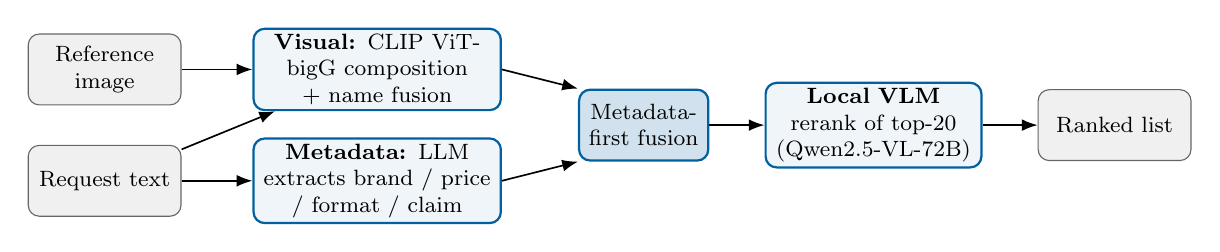
\begin{tikzpicture}[
  font=\footnotesize,
  box/.style={draw=accent, thick, rounded corners, align=center, minimum height=9mm,
              text width=3.0cm, inner sep=2pt, fill=accent!6},
  io/.style={draw=black!60, rounded corners, align=center, minimum height=9mm,
             text width=1.8cm, inner sep=2pt, fill=black!6},
  op/.style={draw=accent, thick, rounded corners, align=center, minimum height=9mm,
             text width=1.5cm, inner sep=2pt, fill=accent!18},
  arr/.style={-{Latex[length=2mm]}, semithick}]
  \node[io] (img) {Reference image};
  \node[io, below=5mm of img] (txt) {Request text};
  \node[box, right=9mm of img] (vis) {\textbf{Visual:} CLIP ViT-bigG composition + name fusion};
  \node[box, right=9mm of txt] (meta) {\textbf{Metadata:} LLM extracts brand / price / format / claim};
  \node[op] (fuse) at ($(vis.east)!0.5!(meta.east)+(1.8cm,0)$) {Metadata-first fusion};
  \node[box, right=7mm of fuse, text width=2.6cm] (rr) {\textbf{Local VLM} rerank of top-20 (Qwen2.5-VL-72B)};
  \node[io, right=7mm of rr] (out) {Ranked list};
  \draw[arr] (img)--(vis); \draw[arr] (txt)--(vis); \draw[arr] (txt)--(meta);
  \draw[arr] (vis.east)--(fuse.north west); \draw[arr] (meta.east)--(fuse.south west);
  \draw[arr] (fuse)--(rr); \draw[arr] (rr)--(out);
\end{tikzpicture}}
\end{center}
\medskip
\footnotesize
\begin{columns}[T]
\begin{column}{0.5\textwidth}
\begin{itemize}
  \item \textbf{Visual}: training-free; no CIR training needed
  \item \textbf{Metadata}: score brand-matched products by price proximity +
        format/claim keywords; abstain if no confident brand
\end{itemize}
\end{column}
\begin{column}{0.5\textwidth}
\begin{itemize}
  \item \textbf{Fusion}: confident metadata hits first, then visual list
  \item \textbf{Rerank}: open-weight VLM served locally with vLLM
\end{itemize}
\end{column}
\end{columns}
\end{frame}

% ------------------------------------------------------------------
\begin{frame}{Finding 1 --- Recall, not reranking, is the bottleneck}
A reranker can only reorder what Stage-1 retrieved. With one gold answer per
Dev query, the best nDCG@10 \emph{any} reranker can reach = the pool's
\textbf{recall} at its depth.
\medskip
\begin{center}\small
\begin{tabular}{@{}lccc@{}}
\toprule
Stage-1 pool (Dev-429) & R@20 & R@50 & Stage-1 nDCG@10 \\
\midrule
SEARLE-Phi (textual inversion) & 0.084 & 0.154 & 0.029 \\
bigG + name fusion (visual)    & 0.359 & 0.436 & 0.157 \\
\textbf{Metadata-fused (ours)} & \textbf{0.431} & \textbf{0.527} & \textbf{0.200} \\
\bottomrule
\end{tabular}
\end{center}
\medskip
\begin{center}\color{accent}
Visual backbones plateau near 0.44 R@50; only metadata breaks it.\\
Improving Stage-1 raises the ceiling; reranker tuning only closes the gap beneath it.
\end{center}
\end{frame}

% ------------------------------------------------------------------
\begin{frame}{Finding 2 --- Price carries the gain; local rerankers are competitive}
\begin{columns}[T]
\begin{column}{0.46\textwidth}
\textbf{Price carries the metadata gain}\\
{\footnotesize Dev, metadata-only, gold fields}
\begin{center}\footnotesize
\begin{tabular}{@{}lc@{}}
\toprule
Terms & nDCG@10 \\ \midrule
brand only        & 0.084 \\
brand + format    & 0.110 \\
\textbf{brand + price} & \textbf{0.232} \\
all four terms    & 0.211 \\
\bottomrule
\end{tabular}
\end{center}
{\footnotesize Full 2{,}083-query Dev set (79\% free-form): 0.115 vs.\ 0.119 for bigG alone --- roughly neutral.}
\end{column}
\begin{column}{0.54\textwidth}
\textbf{Local VLMs are competitive with a hosted API}\\
{\footnotesize same SEARLE-Phi top-20 pool, Official-20 proxy}
\begin{center}\footnotesize
\resizebox{\linewidth}{!}{%
\begin{tabular}{@{}lcc@{}}
\toprule
Reranker & proxy nDCG@10 & marginal cost/pass \\ \midrule
Qwen2.5-VL-72B (local) & 0.913 & $\sim$\$0 \\
InternVL3-38B (local)  & 0.907 & $\sim$\$0 \\
Qwen2.5-VL-32B (local) & 0.894 & $\sim$\$0 \\
Haiku (hosted API)     & 0.872 & $\sim$\$11 \\
Pixtral-Large (local)  & 0.869 & $\sim$\$0 \\
\bottomrule
\end{tabular}}
\end{center}
{\footnotesize Three of four score above the API, but gaps are within proxy noise. $\sim$\$0 is marginal, once a GPU is rented ($\sim$\$60 total).}
\end{column}
\end{columns}
\end{frame}

% ------------------------------------------------------------------
\begin{frame}{Official results}
\begin{columns}[T]
\begin{column}{0.52\textwidth}
\footnotesize
\resizebox{\linewidth}{!}{%
\begin{tabular}{@{}llcc@{}}
\toprule
Run & Stage-1 $\to$ reranker & @5 & @10 \\ \midrule
\textbf{Run1} & \textbf{fused (bigG+meta) $\to$ Qwen-72B} & \textbf{0.740} & \textbf{0.714} \\
Run5 & bigG name-fused+BU $\to$ Qwen-32B & 0.739 & 0.709 \\
Run2 & SEARLE-Phi $\to$ Qwen-72B & 0.680 & 0.636 \\
Run3 & SEARLE-Phi $\to$ InternVL3-38B & 0.650 & 0.628 \\
Run4 & SEARLE-Phi $\to$ Qwen-32B & 0.625 & 0.606 \\
\bottomrule
\end{tabular}}
\smallskip

{\scriptsize Official nDCG on 20 topics, pooled human judgments. BU = symbolic brand-union.}
\end{column}
\begin{column}{0.48\textwidth}
\footnotesize
\begin{itemize}
  \item \textbf{3rd of 5 teams} at both cutoffs; at \textbf{nDCG@10} the top
        four are within \textbf{0.019} --- no ordering inferred among 2nd--4th
  \item \textbf{Same pool, 3 rerankers}: 0.030 apart ($p{\approx}0.52$);
        per-topic up to 0.22
  \item \textbf{Same reranker, new Stage-1}: \textbf{+0.078} (Run2$\to$1),
        \textbf{+0.103} (Run4$\to$5)
\end{itemize}
\end{column}
\end{columns}
\medskip
\begin{center}\color{accent}\small
In aggregate, candidate generation is the larger lever.\\
{\footnotesize The contrasts swap the whole Stage-1 (Run5's brand-union added no official
candidates), so metadata's own effect is shown on Dev.}
\end{center}
\end{frame}

% ------------------------------------------------------------------
\begin{frame}{Takeaways}
\begin{itemize}
  \item \textbf{Recall, not reranking,} caps CIR on a structured e-commerce corpus --- in aggregate; single topics can still be reranker-sensitive.
  \item \textbf{Structured metadata --- especially price ---} recovers what a
        visual encoder cannot see; gains concentrate on structured requests.
  \item \textbf{Local open-weight VLM rerankers} are competitive with a hosted
        API at near-zero marginal cost.
\end{itemize}
\medskip
\footnotesize\textit{Caution:} in one recorded Dev comparison, visually reranking the
metadata pool lowered exact-match nDCG@10 from 0.200 to 0.173; the item-level
mechanism is unverified.\\
\textit{Next:} better brand resolution; repeat the metadata-pool rerank audit before
deciding whether to pin matches; validate extraction on natural official queries.
\vfill
\begin{center}\large\color{accent}
Thank you --- questions?\\[2pt]
\normalsize ale.magnani@gmail.com
\end{center}
\end{frame}

\end{document}
